\documentclass{article}
\usepackage{graphicx}
\usepackage[utf8]{inputenc}
\usepackage{amsmath, amssymb, latexsym}

\usepackage{pgfplots}
\usepackage{algorithm}
\usepackage[noend]{algpseudocode}
\usepackage{tikz}
\usepackage{nicefrac}
\usepackage{placeins}
\pgfplotsset{every axis legend/.append style={
at={(0,0)},
anchor=north east}}
\usetikzlibrary{shapes,positioning,intersections,quotes}
\usetikzlibrary{arrows.meta,
                bending,
                intersections,
                quotes,
                shapes.geometric}
                
\definecolor{darkgreen}{rgb}{0.0, 0.6, 0.0}
\definecolor{darkred}{rgb}{0.7, 0.0, 0.0}
\makeatletter
\def\BState{\State\hskip-\ALG@thistlm}
\makeatother
\title{Week 18}
\begin{document}
\pagenumbering{gobble}
\maketitle
\newpage
\pagenumbering{arabic}

\section*{Problem description and pipeline}

\begin{itemize}
  \item Consider how a complex system may be built.
  \item The idea of a machine learning pipeline.
  \item Machine learning applied to real-world issues and artificial data synthesis.
\end{itemize}

~\\
What is the photo OCR problem?
\begin{itemize}
  \item Photo OCR = photo optical character recognition.
  \item Getting computers to interpret digital images is one notion that has piqued the curiosity of many people.
  \item The idea behind picture OCR is to teach computers to interpret text in images.
\end{itemize}

~\\
Pipeline - a sequence of separate modules, each of which may be a machine learning or data processing component.

~\\
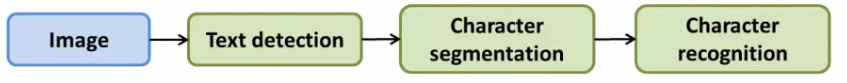
\includegraphics[width=\textwidth]{resources/ocr_pipeline}

\section*{Pedestrian detection}

\begin{itemize}
  \item We're looking for pedestrians in the picture.
  \item A common aspect ratio for a standing human is 82 x 36.
  \item Obtain a training set of both positive and negative examples (1000 - 10 000).
\end{itemize}

~\\
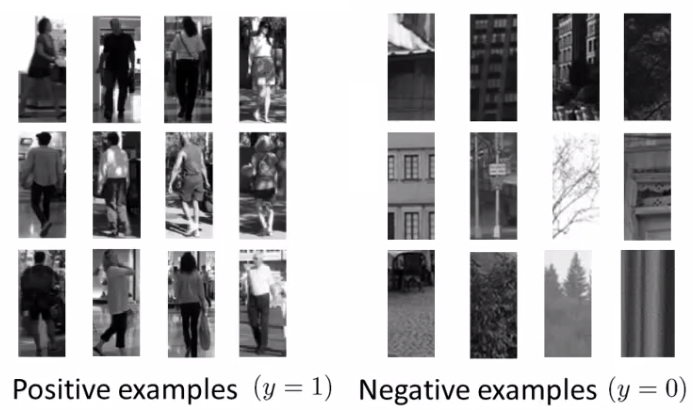
\includegraphics[width=0.8\textwidth]{resources/pedestrians_training_set}

\begin{itemize}
  \item Now that we have a new image, how do we identify pedestrians within it?
  \item Start by taking a rectangular 82 x 36 patch in the image.
  \item Run patch through classifier (returns 1 or 0).
  \item After that, move the rectangle slightly to the right and re-run the program.
  \item Repeat until you've covered the whole image.
  \item Hopefully, by varying the patch size and rastering over the image frequently, you will finally recognize all of the pedestrians in the image.
\end{itemize}

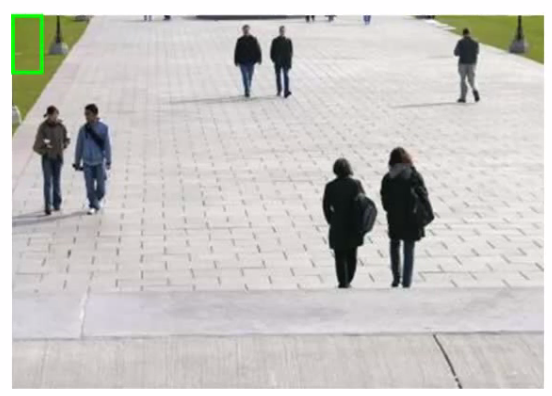
\includegraphics[width=0.7\textwidth]{resources/pedestrians}

\section*{Text detection example}

\begin{itemize}
  \item We generate a labeled training set with positive examples (some type of text) and negative examples (not text), similar to pedestrian detection.
  \item After training the classifier, we apply it to an image using a sliding window classifier with a set rectangle size.
  \item Obtain a training set of both positive and negative examples (1000 - 10 000).
  \item The white region indicates where the text recognition algorithm believes text exists, while the varying shades of gray correlate to the likelihood associated with how certain the classifier is that the section includes text
\end{itemize}

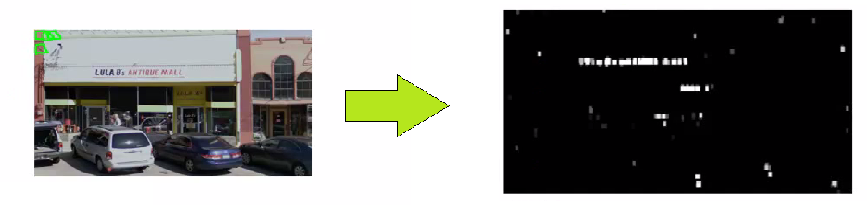
\includegraphics[width=\textwidth]{resources/text_detection}

\begin{itemize}
  \item Take the classifier output and apply an expansion algorithm that extends each of the white areas.
  \item Examine the linked white patches in the picture above. Draw rectangles around those that make sense as text (tall narrow boxes don't).
  \item This example misses a piece of text on the door because the aspect ratio is wrong.
\end{itemize}

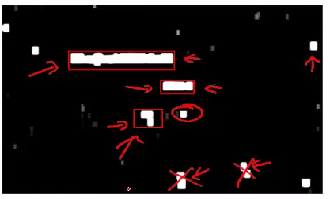
\includegraphics[width=0.6\textwidth]{resources/expansion_algorithm}

\subsection*{Stage two is character segmentation}

\begin{itemize}
  \item To navigate along text areas, use a 1-dimensional sliding window.
  \item Does each window snapshot resemble the separation of two characters?
  \item Insert a split if yes.
  \item If not, proceed.
\end{itemize}
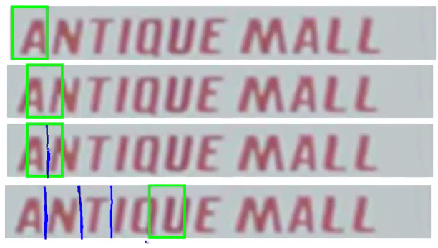
\includegraphics[width=0.5\textwidth]{resources/character_segmentation}

\section*{Character recognition as an example of data synthesis}

\begin{itemize}
  \item The goal is for the system to recognize a character based on an image patch.
  \item Consider the photos to be grayscale (makes it a bit easer).
  \item Where can I find training data?
  \item Modern computers frequently include a large font library, and there are several free font libraries available on the internet.
  \item Take characters from different fonts and place them on random backgrounds to get more training data.
  \item Another approach is to add distortion into existing data, such as warping a character.
\end{itemize}

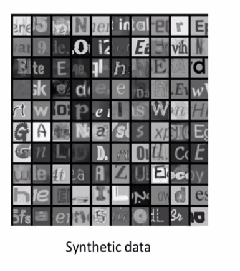
\includegraphics[width=0.5\textwidth]{resources/characters}

\end{document}
